% Provenance (never printed): see sources/outline_sources.md (Year 1: insolation with
% latitude and season, the radiative surplus and deficit, meridional heat transport by
% the atmosphere and the ocean, latent heat). Exercise and problem values in the Book 3
% scratch calculator calc/ch27.py; figures from figdata/bachelor-1/insolation.py (Kepler
% orbit of _solar.py) and energy_balance.py (NCEP-NCAR Reanalysis 1, long-term means
% 1991-2020, datasets bachelor-1-ncep-*).
% Physics owns the inverse-square law, the black body and the Stefan-Boltzmann law, the
% seasons and latent heat (recalled). Book 2 (g10) gave the quarter of the solar constant,
% the global budget diagram and its closure, latent and sensible heat in words, the
% annual-mean insolation curve and the poleward transport in words: re-founded here with
% derivations and data. Ch. 1 gave the instantaneous insolation, the declination and the
% rising and setting of the Sun.
\chapter{Radiação e transporte de calor}\label{ch:b1:radiation-heat-transport}

De um milhão de milhas de distância, a face iluminada da Terra é um disco de mar azul, terra
marrom e nuvem branca. A luz do sol cai mais diretamente no centro do disco, perto dos trópicos,
e roça suas bordas; os trópicos absorvem muito mais energia que as regiões polares. No entanto os
trópicos não se tornam mais quentes ano após ano, nem os polos mais frios. Os ventos e as
correntes oceânicas levam o excesso em direção aos polos, vários petawatts dele. Este capítulo
mede os três termos desse balanço: a luz solar que cada \omterm{def:b1:spherical-astronomy:geographic}{latitude} recebe, a parte que ela retém e
o infravermelho que devolve ao espaço, e o transporte que faz a diferença. Uma grande parcela do
transporte viaja de forma invisível, como vapor d'água, cujo calor latente é liberado onde ele
condensa em chuva.
% ledger: commons:epic-earth, trenberth:transport

\begin{omfigure}
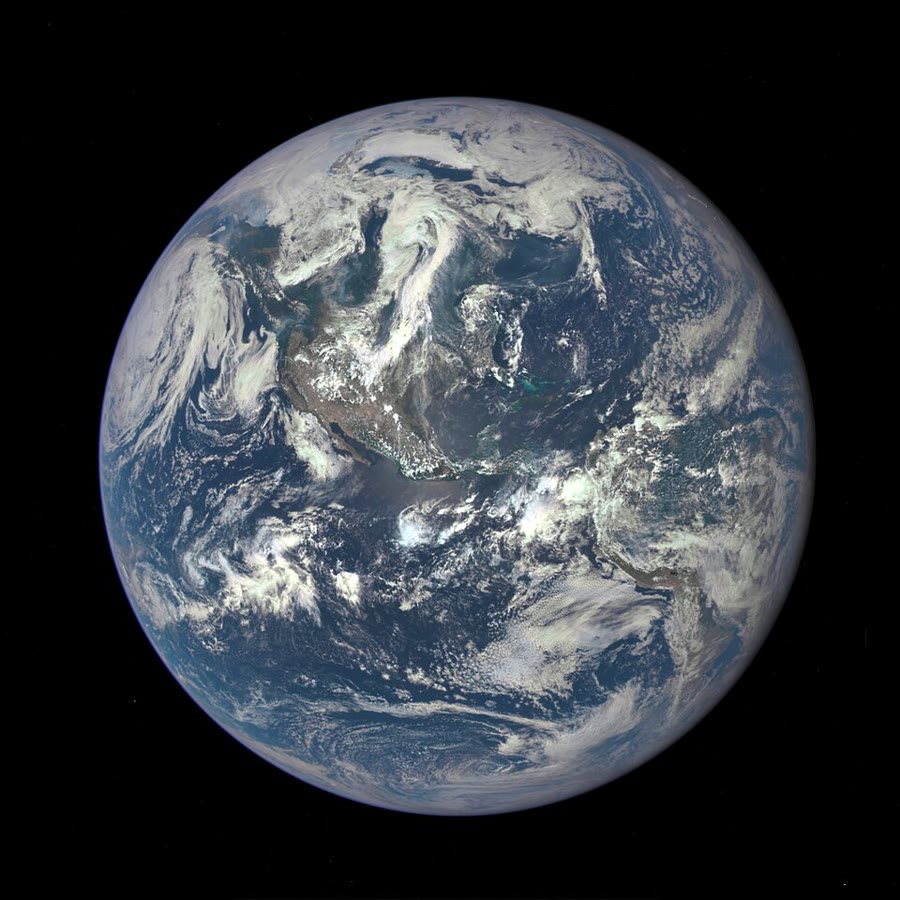
\includegraphics[width=0.55\linewidth]{images/book3/b1-epic-earth.jpg}

{\small A face iluminada inteira da Terra, fotografada em 6 de julho de 2015 por uma câmera do
Deep Space Climate Observatory, a um milhão de milhas de distância; a América do Norte e a
Central estão no meio, com os mares rasos turquesa do Caribe. Duas semanas após o solstício de
junho, o Ártico, no alto, está iluminado durante todo o dia. As nuvens brilhantes refletem grande
parte da luz que as atinge; o tom azulado é a luz solar espalhada pelas moléculas do ar. (NASA
Goddard Space Flight Center, domínio público, via Wikimedia Commons.)}
\label{fig:b1:radiation-heat-transport:epic}
\end{omfigure}
% ledger: commons:epic-earth (polar day: figdata/bachelor-1/insolation.py)

\begin{recall}
\Cref{ch:b1:spherical-astronomy} definiu a \omterm{def:b1:spherical-astronomy:insolation}{insolação}, a potência da luz solar recebida por metro
quadrado de uma superfície horizontal no topo da atmosfera, $I = S_0(a/r)^2\sin h_\odot$ enquanto
o Sol está acima, com $S_0 = \qty{1361}{W.m^{-2}}$ à distância média $a$; deu a altitude do Sol a
partir de seu \omterm{def:b1:spherical-astronomy:equatorial}{ângulo horário} $H$, de sua \omterm{def:b1:spherical-astronomy:equatorial}{declinação} $\delta$ e da \omterm{def:b1:spherical-astronomy:geographic}{latitude} $\varphi$,
$\sin h_\odot = \sin\varphi\sin\delta + \cos\varphi\cos\delta\cos H$; e o \omterm{def:b1:spherical-astronomy:equatorial}{ângulo horário} $H_0$ do
pôr do Sol, $\cos H_0 = -\tan\varphi\tan\delta$ (\cref{prop:b1:spherical-astronomy:rising}).
\Cref{ch:b1:comparative-planetology} definiu o \omterm{def:b1:comparative-planetology:albedo}{albedo de Bond} de um planeta e sua \omterm{def:b1:comparative-planetology:equilibrium-temperature}{temperatura de
equilíbrio}. Os livros de física dão a lei do inverso do quadrado para a luz, a radiação de um corpo
negro, $\sigma T^4$ por metro quadrado com $\sigma = \qty{5.670e-8}{W.m^{-2}.K^{-4}}$
(Stefan--Boltzmann), e o calor latente de uma mudança de estado. O Livro~2 mostrou que a Terra
intercepta em média um quarto da constante solar, desenhou o balanço global de energia da Terra e
verificou que ele se equilibra, e descreveu em palavras o transporte de calor em direção aos polos.
% ledger: earth:TSI, const:sigma, ipcc:budget-toa
\end{recall}

\section{Insolação com a latitude e a estação}\label{sec:b1:radiation-heat-transport:insolation}

A \omterm{def:b1:spherical-astronomy:insolation}{insolação} instantânea muda de minuto a minuto à medida que o Sol cruza o céu. Para o clima, o que
conta é sua soma ao longo de um dia.

\begin{definition}[Insolação média diária]\label{def:b1:radiation-heat-transport:daily-insolation}
A \emph{insolação média diária}\index{insolação média diária} $\bar Q$ em uma \omterm{def:b1:spherical-astronomy:geographic}{latitude} em um dado
dia é a \omterm{def:b1:spherical-astronomy:insolation}{insolação} instantânea média nas 24 horas desse dia, noites incluídas, a \omterm{def:b1:spherical-astronomy:equatorial}{declinação} do Sol
e sua distância sendo mantidas nos valores do dia. É uma potência por metro quadrado de superfície
horizontal no topo da atmosfera, em \unit{W.m^{-2}}.
\end{definition}

Manter $\delta$ e $r$ fixos durante um dia é inofensivo: a \omterm{def:b1:spherical-astronomy:equatorial}{declinação} muda no máximo \ang{0.4} por
dia, e a distância menos de \qty{0.03}{\percent}.
% ledger: earth:obliquity, earth:ecc (computed in figdata/bachelor-1/insolation.py)

\begin{theorem}[Insolação média diária]\label{thm:b1:radiation-heat-transport:daily}
Na \omterm{def:b1:spherical-astronomy:geographic}{latitude} $\varphi$, em um dia em que a \omterm{def:b1:spherical-astronomy:equatorial}{declinação} do Sol é $\delta$ e sua distância $r$,
\[
  \bar Q = \frac{S_0}{\pi}\left(\frac{a}{r}\right)^{2}
  \bigl(h_0\sin\varphi\sin\delta + \cos\varphi\cos\delta\sin h_0\bigr),
\]
onde $h_0 \in [0, \pi]$ é o \omterm{def:b1:spherical-astronomy:equatorial}{ângulo horário} do pôr do Sol em radianos: $\cos h_0 =
-\tan\varphi\tan\delta$ quando $|\tan\varphi\tan\delta| \le 1$; $h_0 = \pi$ no dia polar
($\tan\varphi\tan\delta > 1$); $h_0 = 0$, e $\bar Q = 0$, na noite polar ($\tan\varphi\tan\delta < -1$).
\end{theorem}

\begin{proof}
O \omterm{def:b1:spherical-astronomy:equatorial}{ângulo horário} $H$ avança uniformemente por $2\pi$ em um dia, de modo que a média do dia é a
média sobre $H \in [-\pi, \pi]$. O Sol está acima para $-h_0 < H < h_0$, onde $\sin h_\odot > 0$,
e a \omterm{def:b1:spherical-astronomy:insolation}{insolação} é nula fora disso. Daí
\[
  \bar Q = \frac{1}{2\pi}\int_{-h_0}^{h_0} S_0\left(\frac{a}{r}\right)^{2}
  \bigl(\sin\varphi\sin\delta + \cos\varphi\cos\delta\cos H\bigr)\,\mathrm dH ,
\]
que é $(S_0/2\pi)(a/r)^2\bigl(2h_0\sin\varphi\sin\delta +
2\cos\varphi\cos\delta\sin h_0\bigr)$.
Os limites vêm de \cref{prop:b1:spherical-astronomy:rising}: a altitude é nula quando $\cos H = -\tan\varphi\tan\delta$. Se esse número excede 1 em valor absoluto, o Sol nunca cruza o horizonte:
quando $\tan\varphi\tan\delta > 1$, o integrando é positivo para todo $H$ e a integral percorre o
dia inteiro, $h_0 = \pi$; quando $\tan\varphi\tan\delta < -1$, é negativo para todo $H$ e o Sol
nunca nasce.
\end{proof}

Dois casos especiais valem a pena conhecer de cor. No equador, $\varphi = 0$ e $h_0 = \pi/2$
qualquer que seja a estação:
\[
  \bar Q_\text{equador} = \frac{S_0}{\pi}\left(\frac{a}{r}\right)^{2}\cos\delta ,
\]
maior nos equinócios, $S_0/\pi = \qty{433.2}{W.m^{-2}}$ à distância média. Em um polo no seu verão,
$h_0 = \pi$ e $\varphi = \pi/2$: $\bar Q_\text{polo} =
S_0(a/r)^2\sin\delta$, o Sol dando voltas no céu a uma altitude constante igual à \omterm{def:b1:spherical-astronomy:equatorial}{declinação}.
% ledger: earth:TSI

\begin{proposition}[O verão polar]\label{prop:b1:radiation-heat-transport:polar-summer}
Em um dia de \omterm{def:b1:spherical-astronomy:equatorial}{declinação} $\delta > 0$, a \omterm{def:b1:radiation-heat-transport:daily-insolation}{insolação média diária} no Polo Norte excede a do equador se
e somente se $\pi\tan\delta > 1$, isto é $\delta >
\ang{17.66}$. No solstício de junho, $\delta = \ang{23.44}$, a razão é $\pi\tan
\delta = 1.362$.
\end{proposition}

\begin{proof}
Os dois casos especiais acima compartilham o fator $(S_0/\pi)(a/r)^2$; sua razão é
$\pi\sin\delta/\cos\delta = \pi\tan\delta$, que excede 1 quando $\tan\delta >
1/\pi$, $\delta > \arctan(1/\pi) = \ang{17.66}$. Com a obliquidade, $\pi\tan\ang{23.44} = 1.362$.
\end{proof}
% ledger: earth:obliquity

Com a órbita da Terra, o solstício de junho cai perto do afélio, $(a/r)^2 = 0.968$: o Polo Norte
recebe então \qty{524}{W.m^{-2}} como média diária, o equador \qty{385}{W.m^{-2}}. Seis meses
depois o Polo Sul, perto do periélio, recebe \qty{559}{W.m^{-2}}, \qty{6.7}{\percent} a mais que o
Polo Norte teve em seu verão: a razão é exatamente a dos dois valores de $(a/r)^2$. A figura abaixo
mostra $\bar Q$ ao longo de um ano inteiro. Os máximos estão nos polos nos solstícios; as cunhas
escuras são as noites polares, delimitadas pela \omterm{def:b1:spherical-astronomy:geographic}{latitude} $\ang{90} -
|\delta|$; o ponto subsolar, onde o Sol passa a pino ao meio-dia, se desloca entre os trópicos
com a \omterm{def:b1:spherical-astronomy:equatorial}{declinação}.
% ledger: earth:TSI, earth:ecc, earth:obliquity, nasa:earth-perihelion-longitude, usno:seasons-2026 (computed in figdata/bachelor-1/insolation.py)

\begin{omfigure}
\begin{tikzpicture}
\begin{axis}[omrecord, width=0.8\linewidth, height=6.4cm, view={0}{90},
  xmin=0, xmax=365, ymin=-90, ymax=90, xlabel={dia do ano (a partir de 1º de janeiro)},
  ylabel={latitude (\unit{\degree})}, xtick={0,60,...,360}, ytick={-90,-60,...,90},
  colormap/viridis, colorbar, point meta min=0, point meta max=560,
  colorbar style={ylabel={$\bar Q$ (\unit{W.m^{-2}})}, ytick={0,100,...,500}, width=0.3cm},
  axis on top, grid=none]
% figdata/bachelor-1/insolation.py; ledger: earth:TSI, earth:ecc, earth:obliquity, nasa:earth-perihelion-longitude, usno:tropical-year, usno:seasons-2026
\addplot3[surf, shader=interp, mesh/ordering=y varies, mesh/rows=73]
  table[x=day, y=lat, z=Q] {figdata/out/bachelor-1-insolation-grid.dat};
\addplot3[white, dashed, line width=0.8pt] table[x=day, y=decl, z expr=600] {figdata/out/bachelor-1-insolation-sun.dat};
\addplot3[white, line width=0.6pt, unbounded coords=jump] table[x=day, y=night_n, z expr=600] {figdata/out/bachelor-1-insolation-sun.dat};
\addplot3[white, line width=0.6pt, unbounded coords=jump] table[x=day, y=night_s, z expr=600] {figdata/out/bachelor-1-insolation-sun.dat};
\node[font=\scriptsize, text=white] at (axis cs:28,81,700) {noite polar};
\node[font=\scriptsize, text=white] at (axis cs:172,-81,700) {noite polar};
\node[font=\scriptsize, text=white, anchor=south] at (axis cs:172,26,700) {latitude subsolar};
\end{axis}
\end{tikzpicture}

{\small \omterm{def:b1:radiation-heat-transport:daily-insolation}{Insolação média diária} no topo da atmosfera em função do dia do ano e da \omterm{def:b1:spherical-astronomy:geographic}{latitude}, a partir
de \cref{thm:b1:radiation-heat-transport:daily} com $S_0 = \qty{1361}{W.m^{-2}}$ e a órbita da
Terra. Tracejado: a \omterm{def:b1:spherical-astronomy:geographic}{latitude} subsolar, igual à \omterm{def:b1:spherical-astronomy:equatorial}{declinação}; contínuo: as bordas das noites polares.
Os polos de verão recebem mais que qualquer outro lugar da Terra; o verão austral, perto do
periélio, é o mais brilhante dos dois.}
\label{fig:b1:radiation-heat-transport:matrix}
\end{omfigure}
% ledger: earth:TSI, earth:ecc, earth:obliquity, nasa:earth-perihelion-longitude, usno:seasons-2026

A média de $\bar Q$ ao longo do ano dá a \omterm{def:b1:spherical-astronomy:insolation}{insolação} média anual de cada \omterm{def:b1:spherical-astronomy:geographic}{latitude} (figura abaixo):
\qty{415.6}{W.m^{-2}} no equador, \qty{328.3}{W.m^{-2}} a \ang{40}, \qty{172.4}{W.m^{-2}} em cada
polo. O verão polar é intenso, mas o inverno polar é escuro, e ao longo de um ano o equador recebe
\num{2.41} vezes mais que um polo. A curva é a mesma nos dois hemisférios, embora o verão austral
seja o mais brilhante; \cref{exo:b1:radiation-heat-transport:10} mostra por quê.
% ledger: earth:TSI, earth:ecc, earth:obliquity (computed in figdata/bachelor-1/insolation.py)

\begin{omfigure}
\begin{tikzpicture}
\begin{axis}[omrecord, width=0.8\linewidth, height=5.6cm, xmin=-90, xmax=90, ymin=0, ymax=600,
  xlabel={latitude (\unit{\degree})}, ylabel={$\bar Q$ (\unit{W.m^{-2}})},
  xtick={-90,-60,...,90}, ytick={0,100,...,600}]
% figdata/bachelor-1/insolation.py; ledger: earth:TSI, earth:ecc, earth:obliquity, nasa:earth-perihelion-longitude
\addplot[omThm, line width=0.8pt] table[x=lat, y=Q_jun] {figdata/out/bachelor-1-insolation-annual.dat};
\addplot[omDef, line width=0.8pt] table[x=lat, y=Q_dec] {figdata/out/bachelor-1-insolation-annual.dat};
\addplot[black, line width=1.1pt] table[x=lat, y=Q_ann] {figdata/out/bachelor-1-insolation-annual.dat};
\addplot[black!60, dashed, domain=-90:90] {340.30};
  \node[font=\scriptsize, text=omThm, anchor=west] at (axis cs:50,540) {solstício de junho};
  \node[font=\scriptsize, text=omDef, anchor=east] at (axis cs:-50,575) {solstício de dezembro};
  \node[font=\scriptsize, anchor=north] at (axis cs:-72,160) {média anual};
  \node[font=\scriptsize, text=black!60, anchor=south west] at (axis cs:-88,342) {média global};
\end{axis}
\end{tikzpicture}

{\small \omterm{def:b1:radiation-heat-transport:daily-insolation}{Insolação média diária} contra a \omterm{def:b1:spherical-astronomy:geographic}{latitude} nos dois solstícios, e sua média anual (preta). A
média anual excede a média global, \qty{340.3}{W.m^{-2}} (tracejada), entre \ang{37} S e \ang{37} N,
em \qty{60}{\percent} da superfície da Terra.}
\label{fig:b1:radiation-heat-transport:annual}
\end{omfigure}
% ledger: earth:TSI, earth:ecc, earth:obliquity (computed in figdata/bachelor-1/insolation.py)

\begin{proposition}[A média global]\label{prop:b1:radiation-heat-transport:global}
A cada instante, a \omterm{def:b1:spherical-astronomy:insolation}{insolação} média sobre toda a esfera é $\tfrac14
S_0(a/r)^2$. Média também ao longo do ano, ela é $S_0/(4\sqrt{1 - e^2})$, onde $e$ é a
excentricidade da órbita: \qty{340.30}{W.m^{-2}} para a Terra, a menos de \qty{0.02}{\percent} de
$S_0/4 = \qty{340.25}{W.m^{-2}}$.
\end{proposition}

\begin{proof}
A Terra, de raio $R$, intercepta a luz solar que atravessa um disco de área $\pi
R^2$, uma potência $S_0(a/r)^2\pi R^2$, que cai sobre o hemisfério do dia; espalhada por toda a
superfície $4\pi R^2$, ela dá o primeiro resultado. A média no tempo de $(a/r)^2$ sobre a órbita é
$1/\sqrt{1-e^2}$ (\cref{exo:b1:radiation-heat-transport:11}).
\end{proof}
% ledger: earth:TSI, earth:ecc

\section{Radiação absorvida e emitida}\label{sec:b1:radiation-heat-transport:toa}

Da luz solar que uma \omterm{def:b1:spherical-astronomy:geographic}{latitude} recebe, ela reflete uma fração de volta diretamente, pelas nuvens,
neve, gelo, deserto e, em menor grau, pelo mar; absorve o resto, no ar e na superfície. Ela também
perde energia emitindo radiação infravermelha para o espaço, de dia e de noite.

\begin{definition}[Radiação de onda longa emitida]\label{def:b1:radiation-heat-transport:olr}
A \emph{radiação de onda longa emitida}\index{radiação de onda longa emitida} (OLR) é a potência da
radiação infravermelha que deixa o topo da atmosfera rumo ao espaço, por metro quadrado. A
\emph{temperatura de emissão}\index{temperatura de emissão} $T_e$ é a temperatura de um corpo
negro que emitiria a mesma potência:
$\sigma T_e^4 = \text{OLR}$.
\end{definition}

A OLR vem em parte da superfície, através do ar onde ele é transparente ao infravermelho, e em
parte do ar e do topo das nuvens mais altos. A \omterm{def:b1:radiation-heat-transport:olr}{temperatura de emissão} é uma propriedade da
radiação, não a temperatura de um nível particular: ela é menor que a do solo abaixo, porque as
camadas que emitem são mais frias.
% ledger: ipcc:budget-surface, ipcc:budget-toa

\begin{definition}[Radiação líquida; excedente e déficit radiativos]\label{def:b1:radiation-heat-transport:net-radiation}
A \emph{radiação líquida}\index{radiação líquida} no topo da atmosfera é
\[
  R = \underbrace{(1 - \alpha)\,\bar Q}_{\text{solar absorvida}} - \text{OLR},
\]
onde $\alpha$ é o albedo local, a fração da luz solar incidente refletida para o espaço; as três
grandezas são médias anuais em uma \omterm{def:b1:spherical-astronomy:geographic}{latitude}. Uma \omterm{def:b1:spherical-astronomy:geographic}{latitude} onde $R > 0$ tem um
\emph{excedente radiativo}\index{excedente radiativo}; uma onde $R < 0$ tem um
\emph{déficit radiativo}\index{déficit radiativo}.
\end{definition}

Em toda a Terra a \omterm{def:b1:radiation-heat-transport:net-radiation}{radiação líquida} deve ter média quase nula, já que o planeta não se aquece nem se
resfria mais que algumas décimas de watt por metro quadrado: a avaliação mais recente põe o
desequilíbrio em \qty{0.7}{W.m^{-2}}, sobre uma entrada de \qty{340}{W.m^{-2}} dos quais
\qty{100}{W.m^{-2}} são refletidos (um albedo global de \num{0.294}) e \qty{239}{W.m^{-2}} saem
como infravermelho.
% ledger: ipcc:budget-toa, earth:albedo

Os perfis zonais deste capítulo vêm de uma reanálise, isto é, um sistema de previsão do tempo rodado
nas últimas décadas, que assimila as observações de cada dia e produz um estado completo e coerente
da atmosfera. A reanálise usada aqui, desde 1948, dá médias mensais em uma grade de 94 \omterm{def:b1:spherical-astronomy:geographic}{latitudes} e
192 \omterm{def:b1:spherical-astronomy:geographic}{longitudes}; este capítulo usa suas médias de 1991--2020. Seus fluxos de radiação são saídas de
modelo, previsões restringidas pelas observações. A figura abaixo mostra suas médias zonais contra
$\sin\varphi$, de modo que larguras iguais no eixo são áreas iguais na esfera.
% ledger: psl:ncep-r1, kalnay96:reanalysis, data:b3-ncep

\begin{omfigure}
\begin{tikzpicture}
\begin{axis}[omrecord, width=0.8\linewidth, height=6cm, xmin=-1, xmax=1, ymin=0, ymax=320,
  xlabel={latitude (\unit{\degree}, eixo em $\sin\varphi$)}, ylabel={fluxo (\unit{W.m^{-2}})},
  xtick={-0.866,-0.5,0,0.5,0.866}, xticklabels={60 S,30 S,0,30 N,60 N},
  ytick={0,50,...,300}]
% figdata/bachelor-1/energy_balance.py; ledger: data:b3-ncep, psl:ncep-r1
\addplot[name path=asr, omProp, line width=1pt] table[x expr={sin(\thisrow{lat})}, y=asr] {figdata/out/bachelor-1-energy_balance-toa.dat};
\addplot[name path=olr, omThm, line width=1pt] table[x expr={sin(\thisrow{lat})}, y=olr] {figdata/out/bachelor-1-energy_balance-toa.dat};
\addplot[omProp!25] fill between[of=asr and olr, split, every segment no 1/.style={omDef!18}, every segment no 2/.style={omProp!30}, every segment no 3/.style={omDef!18}];
\node[font=\scriptsize, text=omProp!80!black] at (axis cs:-0.55,300) {solar absorvida};
\node[font=\scriptsize, text=omThm] at (axis cs:-0.2,226) {OLR};
\node[font=\scriptsize] at (axis cs:0,262) {excedente};
\node[font=\scriptsize] at (axis cs:0.86,178) {déficit};
\node[font=\scriptsize] at (axis cs:-0.86,178) {déficit};
\end{axis}
\end{tikzpicture}

{\small Absorção solar média zonal e anual (laranja) e \omterm{def:b1:radiation-heat-transport:olr}{radiação de onda longa emitida} (vermelho) no
topo da atmosfera, a partir da Reanálise~1 NCEP-NCAR, médias 1991--2020 (dados fornecidos pelo NOAA
PSL, Boulder, Colorado, EUA, em seu site https://psl.noaa.gov). Sombreado: o \omterm{def:b1:radiation-heat-transport:net-radiation}{excedente radiativo} das
\omterm{def:b1:spherical-astronomy:geographic}{latitudes} baixas e os déficits das altas \omterm{def:b1:spherical-astronomy:geographic}{latitudes}.}
\label{fig:b1:radiation-heat-transport:toa}
\end{omfigure}
% ledger: data:b3-ncep, psl:ncep-r1, kalnay96:reanalysis

As duas curvas têm formas muito diferentes. A luz solar absorvida cai de \qty{288}{W.m^{-2}} perto
do equador para \qty{76}{W.m^{-2}} a \ang{81} N, por um fator de \num{3.8}: a \omterm{def:b1:spherical-astronomy:insolation}{insolação} diminui, e
o albedo sobe de \num{0.31} para \num{0.57}, com o Sol baixo, a neve e o gelo marinho. A OLR cai
apenas de \qty{245}{W.m^{-2}} para \qty{192}{W.m^{-2}}, por um fator de \num{1.27}; as \omterm{def:b1:radiation-heat-transport:olr}{temperaturas
de emissão} são \qty{256}{K} e \qty{241}{K}. A OLR é até ligeiramente menor no equador,
\qty{245}{W.m^{-2}}, que perto de \ang{20}, \qty{269}{W.m^{-2}}: as nuvens do cinturão equatorial
de chuvas sobem alto e seus topos frios emitem pouco, enquanto os céus subtropicais mais claros
deixam escapar mais infravermelho. Onde a luz solar absorvida excede a OLR, a \omterm{def:b1:spherical-astronomy:geographic}{latitude} tem um
excedente.
% ledger: data:b3-ncep (values computed in figdata/bachelor-1/energy_balance.py)

\begin{example}[O balanço global da reanálise]\label{ex:b1:radiation-heat-transport:global}
Médias sobre o globo, a reanálise recebe \qty{341.9}{W.m^{-2}}, reflete \qty{117.0}{W.m^{-2}} (um
albedo de \num{0.342}), absorve \qty{224.8}{W.m^{-2}} e emite \qty{237.7}{W.m^{-2}}: uma \omterm{def:b1:radiation-heat-transport:net-radiation}{radiação
líquida} de \qty{-12.9}{W.m^{-2}}. A OLR está a menos de \qty{1.3}{W.m^{-2}} dos \qty{239}{W.m^{-2}}
avaliados, mas a reflexão é \qty{17}{W.m^{-2}} maior que os \qty{100}{W.m^{-2}} avaliados. Um
desequilíbrio real desse tamanho resfriaria a Terra em \qty{6.6}{PW}; é um erro do modelo, não uma
propriedade da Terra, e o transporte abaixo é calculado depois de remover a média global.
% ledger: data:b3-ncep, ipcc:budget-toa (computed in figdata/bachelor-1/energy_balance.py)
\end{example}

\section{Transporte meridional de calor}\label{sec:b1:radiation-heat-transport:transport}

\begin{definition}[Transporte meridional de calor]\label{def:b1:radiation-heat-transport:mht}
O \emph{transporte meridional de calor}\index{transporte meridional de calor} $T(\varphi)$ através
do paralelo de \omterm{def:b1:spherical-astronomy:geographic}{latitude} $\varphi$ é a energia levada para o norte através desse paralelo por unidade
de tempo, pela atmosfera e pelo oceano juntos, na média anual. Conta-se positivamente para o norte e
mede-se em petawatts (\qty{1}{PW} = \qty{e15}{W}).
\end{definition}

\begin{proposition}[Transporte a partir da radiação líquida]\label{prop:b1:radiation-heat-transport:mht}
Se a energia armazenada em cada faixa de \omterm{def:b1:spherical-astronomy:geographic}{latitude} não muda de um ano para o outro, então, para uma
Terra de raio $a_\oplus$,
\[
  T(\varphi) = 2\pi a_\oplus^2\int_{-\pi/2}^{\varphi} R(\varphi')\cos\varphi'\,
  \mathrm d\varphi' = -2\pi a_\oplus^2\int_{\varphi}^{\pi/2} R(\varphi')\cos
  \varphi'\,\mathrm d\varphi' ,
\]
e $T$ é extremo nas \omterm{def:b1:spherical-astronomy:geographic}{latitudes} onde $R$ muda de sinal.
\end{proposition}

\begin{proof}
Tome a calota polar ao sul do paralelo $\varphi$ como um volume de controle, do fundo do oceano ao
topo da atmosfera (figura abaixo). A energia entra ou sai dele de apenas duas maneiras: como
radiação no topo, uma potência líquida $\int R\,\mathrm dA$, e pelo transporte através de sua borda,
$-T(\varphi)$ (um transporte para o norte deixa a calota sul). A faixa entre $\varphi'$ e
$\varphi' + \mathrm d\varphi'$ tem área $\mathrm dA = 2\pi a_\oplus\cos\varphi'
\cdot a_\oplus\,\mathrm d\varphi'$. Sem mudança de armazenamento, a soma é nula:
$\int_{-\pi/2}^{\varphi} R\,2\pi a_\oplus^2\cos\varphi'\,\mathrm d\varphi' -
T(\varphi) = 0$. Aplicado à Terra inteira ($\varphi = \pi/2$, sem borda), o mesmo balanço dá
$\int R\,\mathrm dA = 0$ sobre a esfera, daí a segunda forma. Derivando, $T'(\varphi) = 2\pi a_\oplus^2 R(\varphi)\cos\varphi$, que se anula onde $R$ muda de sinal.
\end{proof}
% ledger: earth:Rmean

\begin{omfigure}
\begin{tikzpicture}[>={Stealth[length=2mm]}, font=\scriptsize]
  \def\R{2.0}
  \def\ph{40}
  \fill[omDef!12] ({-\R*cos(\ph)},{\R*sin(\ph)}) arc[start angle=180-\ph, end angle=\ph, radius=\R]
     -- ({\R*cos(\ph)},{\R*sin(\ph)}) arc[start angle=0, end angle=-180, x radius={\R*cos(\ph)}, y radius={0.25*\R*cos(\ph)}] -- cycle;
  \draw[thick] (0,0) circle (\R);
  \draw[black!40] (-\R,0) arc[start angle=180, end angle=360, x radius=\R, y radius={0.25*\R}];
  \draw[black!40, dashed] (\R,0) arc[start angle=0, end angle=180, x radius=\R, y radius={0.25*\R}];
  \draw[omDef, thick] ({-\R*cos(\ph)},{\R*sin(\ph)}) arc[start angle=180, end angle=360, x radius={\R*cos(\ph)}, y radius={0.25*\R*cos(\ph)}];
  \draw[omDef, thick, dashed] ({\R*cos(\ph)},{\R*sin(\ph)}) arc[start angle=0, end angle=180, x radius={\R*cos(\ph)}, y radius={0.25*\R*cos(\ph)}];
  \node[anchor=west, black!60] at (\R+0.05,0) {equador};
  \node[anchor=west, omDef] at ({\R*cos(\ph)+0.1},{\R*sin(\ph)}) {paralelo $\varphi$};
  \foreach \x in {-0.55,0.55} \draw[->, very thick, omProp] (\x,{\R*sin(\ph)-0.75}) -- (\x,{\R*sin(\ph)-0.1});
  \node[omProp!80!black, anchor=east] at ({-\R-0.1},{\R*sin(\ph)-0.4}) {$T(\varphi)$ atravessa a borda};
  \foreach \a in {65,90,115} {
    \draw[->, omThm, decorate, decoration={snake, amplitude=0.6mm, segment length=2mm, post length=1.5mm}]
      ({(\R+0.05)*cos(\a)},{(\R+0.05)*sin(\a)}) -- ({(\R+0.75)*cos(\a)},{(\R+0.75)*sin(\a)});
  }
  \node[omThm, anchor=south] at (0,\R+0.8) {radiação líquida $R < 0$ sobre a calota};
\end{tikzpicture}

{\small O volume de controle de \cref{prop:b1:radiation-heat-transport:mht}, desenhado para a calota
ao norte do paralelo $\varphi$ (sombreada): em regime permanente, o que a calota perde por radiação
no topo da atmosfera (vermelho) é o que a atmosfera e o oceano trazem através de sua borda
(laranja).}
\label{fig:b1:radiation-heat-transport:cap}
\end{omfigure}

Aplicada à reanálise, com a média global de \qty{-12.9}{W.m^{-2}} subtraída de $R$ em cada \omterm{def:b1:spherical-astronomy:geographic}{latitude},
a proposição dá a curva abaixo. O transporte é para o norte no hemisfério norte e para o sul no
hemisfério sul, sempre em direção ao polo. Ele atinge o máximo de \qty{4.1}{PW} perto de \ang{38} N
e \qty{4.5}{PW} perto de \ang{32} S, onde $R$ menos sua média muda de sinal; a \ang{40} N ele vale
\qty{4.11}{PW}. É pequeno no equador, onde o excedente de cada hemisfério é exportado para seu
próprio polo.
% ledger: data:b3-ncep (computed in figdata/bachelor-1/energy_balance.py)

\begin{omfigure}
\begin{tikzpicture}
\begin{axis}[omrecord, width=0.8\linewidth, height=6cm, xmin=-90, xmax=90, ymin=-5.5, ymax=6.4,
  xlabel={latitude (\unit{\degree})}, ylabel={transporte para o norte (\unit{PW})},
  xtick={-90,-60,...,90}, ytick={-4,-2,...,4}]
% figdata/bachelor-1/energy_balance.py; ledger: data:b3-ncep, trenberth:transport
\addplot[black!40, domain=-90:90] {0};
\addplot[black, line width=1.1pt] table[x=lat, y=T_PW] {figdata/out/bachelor-1-energy_balance-transport.dat};
\addplot[omMeth, dashed, line width=0.9pt] table[x=lat, y=T_PW] {figdata/out/bachelor-1-energy_balance-latent.dat};
\addplot[only marks, mark=square*, mark size=2pt, omThm] coordinates {(43,5.0)};
\node[font=\scriptsize, anchor=east] at (axis cs:28,4.4) {total};
  \node[font=\scriptsize, text=omMeth, anchor=north] at (axis cs:42,0.9) {calor latente};
  \node[font=\scriptsize, text=omThm, anchor=south] at (axis cs:43,5.2) {só a atmosfera (Trenberth e Caron)};
\end{axis}
\end{tikzpicture}

{\small O \omterm{def:b1:radiation-heat-transport:mht}{transporte meridional de calor} implicado pela \omterm{def:b1:radiation-heat-transport:net-radiation}{radiação líquida} da reanálise (preto) e sua
parte de calor latente (verde tracejado, da evaporação e da precipitação,
\cref{sec:b1:radiation-heat-transport:latent}); Reanálise~1 NCEP-NCAR, médias 1991--2020, dados
fornecidos pelo NOAA PSL. Quadrado: o transporte apenas da atmosfera numa estimativa restringida
por medidas de satélite da radiação, \qty{5.0}{PW} a \ang{43} N (Trenberth e Caron, 2001).}
\label{fig:b1:radiation-heat-transport:transport}
\end{omfigure}
% ledger: data:b3-ncep, psl:ncep-r1, trenberth:transport

O quadrado na figura é um aviso. Um estudo dos anos 1985--1989, quando um experimento de satélite
mediu a radiação no topo da atmosfera de modo confiável, calculou o transporte da atmosfera a partir
dos ventos, temperaturas e umidade de duas reanálises: a atmosfera sozinha transporta \qty{5.0}{PW}
a \ang{43} N, mais que os \qty{4.0}{PW} desta reanálise para a atmosfera e o oceano juntos. O mesmo
estudo constatou que os fluxos gerados pelo modelo da reanálise concordam menos bem com estimativas
independentes do oceano do que os fluxos derivados das observações. Removida a média global, o
transporte depende apenas de como $R$ varia com a \omterm{def:b1:spherical-astronomy:geographic}{latitude}, e a \omterm{def:b1:radiation-heat-transport:net-radiation}{radiação líquida} desta reanálise
varia pouco demais dos trópicos aos polos. A forma da curva, seus picos nas \omterm{def:b1:spherical-astronomy:geographic}{latitudes} médias e sua
quase simetria, pode ser confiável; sua altura fica pelo menos um quinto aquém.
% ledger: trenberth:transport, tc01:method, data:b3-ncep (computed in figdata/bachelor-1/energy_balance.py)

Quem leva o calor? O mesmo estudo constata que o oceano leva mais que a atmosfera apenas entre o
equador e \ang{17} N; a \ang{35}, onde o transporte total atinge o máximo em cada hemisfério, a
atmosfera leva \qty{78}{\percent} dele no norte e \qty{92}{\percent} no sul. A parcela do oceano é o
assunto de \cref{ch:b1:ocean-circulation}, a da atmosfera de \cref{ch:b1:atmospheric-circulation}.
% ledger: trenberth:transport

\begin{method}[Transporte a partir de faixas zonais]\label{met:b1:radiation-heat-transport:bands}
\begin{enumerate}
  \item Divida a calota a polo da \omterm{def:b1:spherical-astronomy:geographic}{latitude} de interesse em faixas; para cada uma, tome a \omterm{def:b1:spherical-astronomy:insolation}{insolação}
        média $\bar Q_i$, o albedo $\alpha_i$ e a OLR$_i$.
  \item Calcule a \omterm{def:b1:radiation-heat-transport:net-radiation}{radiação líquida} de cada faixa, $R_i = (1 - \alpha_i)\bar Q_i -
        \text{OLR}_i$, e subtraia a média global de $R$ se ela não for nula.
  \item Calcule a área de cada faixa, $A_i = 2\pi a_\oplus^2(\sin\varphi_{i,2} -
        \sin\varphi_{i,1})$, com $a_\oplus = \qty{6371}{km}$.
  \item O transporte através da borda é menos a potência líquida da calota, $-\sum_i R_i A_i$,
        positivo em direção ao polo; divida por \num{e15} para petawatts.
\end{enumerate}
\end{method}
% ledger: earth:Rmean

\section{Calor latente e sensível}\label{sec:b1:radiation-heat-transport:latent}

A superfície da Terra absorve a maior parte da luz solar, mas a atmosfera irradia a maior parte do
infravermelho para o espaço. A superfície entrega energia ao ar de três maneiras: por sua própria
radiação infravermelha, aquecendo o ar em contato com ela, e evaporando água, cujo calor latente é
liberado onde o vapor condensa. Esse lugar pode estar a milhares de quilômetros de distância: o
calor latente viaja com o vento.

\begin{definition}[Fluxos de calor latente e sensível; razão de Bowen]\label{def:b1:radiation-heat-transport:surface-fluxes}
O \emph{fluxo de calor latente}\index{fluxo de calor latente} $LE$ é a potência por metro quadrado
que a superfície perde por evaporação: a taxa de evaporação $E$, em \unit{kg.m^{-2}.s^{-1}}, vezes
o calor latente de vaporização $L$. O \emph{fluxo de calor sensível}\index{fluxo de calor sensível}
$H$ é a potência por metro quadrado que a superfície passa para o ar por condução e turbulência,
aquecendo-o. Ambos são contados positivamente para cima. Sua razão $B = H/LE$ é a
\emph{razão de Bowen}\index{razão de Bowen}.
\end{definition}

Perto de \qty{15}{\celsius}, $L = \qty{2.4655}{MJ.kg^{-1}}$. A \omterm{def:b1:radiation-heat-transport:surface-fluxes}{razão de Bowen} é pequena sobre o mar
e sobre o solo úmido, onde a água é abundante, e grande sobre a terra seca. Na reanálise ela vale
\num{0.09} no equador, \num{0.37} a \ang{25} N, a \omterm{def:b1:spherical-astronomy:geographic}{latitude} dos grandes desertos quentes, e é
negativa a \ang{70} N, onde as superfícies de neve e gelo estão, na média anual, mais frias que o ar
acima delas, de modo que o calor sensível desce. Médio sobre o globo, a reanálise dá $LE =
\qty{82.5}{W.m^{-2}}$ e $H = \qty{15.2}{W.m^{-2}}$, uma \omterm{def:b1:radiation-heat-transport:surface-fluxes}{razão de Bowen} de \num{0.18}; os valores
avaliados são \qty{82}{W.m^{-2}} e \qty{21}{W.m^{-2}}, uma razão de \num{0.26}.
% ledger: nist:water-latent, data:b3-ncep, ipcc:budget-surface (computed in figdata/bachelor-1/energy_balance.py)

O Livro~2 transformou o \omterm{def:b1:radiation-heat-transport:surface-fluxes}{fluxo de calor latente} em uma profundidade de água evaporada por ano. O
inverso transforma uma chuva, que um pluviômetro pode coletar, em um fluxo de energia.

\begin{proposition}[Precipitação como fluxo de energia]\label{prop:b1:radiation-heat-transport:rain}
Uma taxa de precipitação de \qty{1}{m} de água por ano libera na atmosfera, onde seu vapor
condensou, uma potência média de
\[
  \frac{\qty{1000}{kg.m^{-2}} \times \qty{2.4655e6}{J.kg^{-1}}}{\qty{3.156e7}{s}}
  = \qty{78.1}{W.m^{-2}} .
\]
\end{proposition}

\begin{proof}
Uma camada de água de \qty{1}{m} de profundidade tem massa de \qty{1000}{kg} por metro quadrado.
Condensar o vapor que a forma libera $1000L$; um ano de \num{365.25} dias dura \qty{3.156e7}{s}.
\end{proof}
% ledger: nist:water-latent

\begin{example}[O ciclo da água como fluxo de energia]\label{ex:b1:radiation-heat-transport:rain}
O ciclo global da água traz ao oceano \num{373000} quilômetros cúbicos de chuva e neve a cada ano, e
\num{113000} à terra: distribuídos pelos \qty{5.10e8}{km^2} da Terra, dão \qty{0.953}{m} por ano, o
que libera \qty{74}{W.m^{-2}} pela \cref{prop:b1:radiation-heat-transport:rain}. A reanálise chove
\qty{2.82}{mm} por dia, \qty{1.03}{m} por ano, \qty{80}{W.m^{-2}}. Ambos estão próximos do \omterm{def:b1:radiation-heat-transport:surface-fluxes}{fluxo de
calor latente} avaliado, de \qty{82}{W.m^{-2}}, cuja faixa de incerteza é \qtyrange{72}{85}{W.m^{-2}}:
ao longo dos anos, a água que evapora volta a cair, e o calor latente retirado da superfície é todo
entregue ao ar.
% ledger: trenberth:water-cycle, earth:Rmean, data:b3-ncep, ipcc:budget-surface (computed in calc/ch27.py)
\end{example}

O balanço vale para o globo, não para cada \omterm{def:b1:spherical-astronomy:geographic}{latitude}, e a diferença é um transporte (figura abaixo).
Nos subtrópicos o mar evapora mais água do que cai ali: $LE$ excede $LP$, o calor latente da
precipitação. O cinturão equatorial de chuvas e as \omterm{def:b1:spherical-astronomy:geographic}{latitudes} médias recebem mais chuva do que
evaporam. Entre os dois, o vapor é levado pelo vento, e com ele o calor latente. Pelo argumento de
\cref{prop:b1:radiation-heat-transport:mht}, aplicado à integral de $LE - LP$, a reanálise leva
\qty{1.4}{PW} de calor latente para o norte através de \ang{40} N, um terço de seu transporte total
ali; o transporte latente está desenhado tracejado na figura de transporte acima.
% ledger: data:b3-ncep (computed in figdata/bachelor-1/energy_balance.py)

\begin{omfigure}
\begin{tikzpicture}
\begin{axis}[omrecord, width=0.8\linewidth, height=6cm, xmin=-1, xmax=1, ymin=-60, ymax=200,
  xlabel={latitude (\unit{\degree}, eixo em $\sin\varphi$)}, ylabel={fluxo (\unit{W.m^{-2}})},
  xtick={-0.866,-0.5,0,0.5,0.866}, xticklabels={60 S,30 S,0,30 N,60 N},
  ytick={-50,0,50,...,200}]
% figdata/bachelor-1/energy_balance.py; ledger: data:b3-ncep, nist:water-latent
\addplot[black!40, domain=-1:1] {0};
\addplot[omMeth, line width=1pt] table[x expr={sin(\thisrow{lat})}, y=lh] {figdata/out/bachelor-1-energy_balance-surface.dat};
\addplot[omDef, line width=1pt] table[x expr={sin(\thisrow{lat})}, y=lp] {figdata/out/bachelor-1-energy_balance-surface.dat};
\addplot[omThm, dashed, line width=0.9pt] table[x expr={sin(\thisrow{lat})}, y=sh] {figdata/out/bachelor-1-energy_balance-surface.dat};
\node[font=\scriptsize, text=omMeth, anchor=south] at (axis cs:-0.35,118) {$LE$};
\node[font=\scriptsize, text=omDef, anchor=south] at (axis cs:0.06,168) {$LP$};
\node[font=\scriptsize, text=omThm, anchor=south] at (axis cs:0.2,24) {$H$};
\end{axis}
\end{tikzpicture}

{\small Médias zonais e anuais do \omterm{def:b1:radiation-heat-transport:surface-fluxes}{fluxo de calor latente} $LE$ (verde), do calor latente liberado
pela precipitação, $LP$ (azul), e do \omterm{def:b1:radiation-heat-transport:surface-fluxes}{fluxo de calor sensível} $H$ (vermelho, tracejado), a partir da
Reanálise~1 NCEP-NCAR, médias 1991--2020 (dados fornecidos pelo NOAA PSL). Onde $LE > LP$, nos
subtrópicos, vapor d'água é exportado; onde $LP > LE$, sob os cinturões de chuva, ele é importado.}
\label{fig:b1:radiation-heat-transport:surface}
\end{omfigure}
% ledger: data:b3-ncep, psl:ncep-r1, nist:water-latent

\section{O balanço de energia da superfície}\label{sec:b1:radiation-heat-transport:surface}

O balanço global desenhado no Livro~2 pode ser lido como uma equação para a superfície.

\begin{proposition}[Balanço de energia da superfície]\label{prop:b1:radiation-heat-transport:surface}
Seja $R_n$ a \omterm{def:b1:radiation-heat-transport:net-radiation}{radiação líquida} na superfície, a luz solar absorvida mais o infravermelho recebido do
ar menos o infravermelho emitido, e $G$ a potência por metro quadrado que vai para o solo ou o
oceano abaixo. Então, por metro quadrado,
\[
  R_n = LE + H + G .
\]
Na média global, $R_n = 160 + 342 - 398 = \qty{104}{W.m^{-2}}$, dos quais \qty{82}{W.m^{-2}} vão
para a evaporação, \qty{21}{W.m^{-2}} para o \omterm{def:b1:radiation-heat-transport:surface-fluxes}{fluxo de calor sensível}, e $G \approx \qty{1}{W.m^{-2}}$,
dentro do arredondamento dos números, para o oceano e o solo.
\end{proposition}

\begin{proof}
Tome como sistema uma camada fina na superfície, sem capacidade térmica própria. A energia chega a
ela apenas como radiação ($R_n$, líquida) e sai dela apenas como os fluxos latente e sensível para
cima e a condução ou mistura para baixo; o balanço é a equação. Os números são as médias globais
avaliadas.
\end{proof}
% ledger: ipcc:budget-surface

\begin{omfigure}
\begin{tikzpicture}[font=\scriptsize, >={Stealth[length=2.2mm, width=2mm]}, line width=1.3pt]
  \fill[omExo!35] (0,0) rectangle (9.6,0.6);
  \fill[omDef!10] (0,0.6) rectangle (9.6,4.2);
  \draw[thin, black!60] (0,0.6) -- (9.6,0.6);
  \node[anchor=west, black!70] at (0.1,0.3) {solo e oceano};
  \node[anchor=west, black!70] at (0.1,3.9) {atmosfera};
  \draw[->, omProp!90!black] (1.6,3.4) -- (1.6,0.65);
  \node[anchor=east, align=right] at (1.5,2.2) {160\\luz solar\\absorvida};
  \draw[->, omThm!50] (2.6,3.4) -- (2.6,0.65);
  \node[anchor=west, align=left] at (2.7,2.2) {342\\infravermelho\\do ar};
  \draw[->, omThm!80!black] (4.8,0.65) -- (4.8,3.4);
  \node[anchor=west, align=left] at (4.9,2.2) {398\\emitido};
  \draw[->, omMeth!80!black] (6.9,0.65) -- (6.9,3.4);
  \node[anchor=west, align=left] at (7.0,2.6) {82 $LE$};
  \draw[->, omMeth!80!black] (8.2,0.65) -- (8.2,2.0);
  \node[anchor=west, align=left] at (8.3,1.6) {21 $H$};
  \draw[->, black!70] (5.9,0.55) -- (5.9,-0.35);
  \node[anchor=west] at (6.0,-0.15) {$G \approx 1$};
  \draw[thin, black!50, decorate, decoration={brace, amplitude=4pt}] (1.0,4.35) -- (5.2,4.35)
     node[midway, above=3pt, black] {$R_n = 160 + 342 - 398 = 104$};
  \draw[thin, black!50, decorate, decoration={brace, amplitude=4pt}] (6.6,4.35) -- (9.3,4.35)
     node[midway, above=3pt, black] {$LE + H + G = 104$};
\end{tikzpicture}

{\small O balanço médio global de energia da superfície em \unit{W.m^{-2}}, a partir dos valores do
Sexto Relatório de Avaliação do IPCC, Grupo de Trabalho~I, Figura~7.2. A \omterm{def:b1:radiation-heat-transport:net-radiation}{radiação líquida} absorvida
pela superfície, \qty{104}{W.m^{-2}}, é entregue à atmosfera sobretudo como calor latente; $G$, o
pequeno resto, aquece o oceano.}
\label{fig:b1:radiation-heat-transport:budget}
\end{omfigure}
% ledger: ipcc:budget-surface, ipcc:heating

O \omterm{def:b1:radiation-heat-transport:surface-fluxes}{fluxo de calor latente}, quatro quintos de $R_n$, é de longe o maior dos dois termos não
radiativos: sobre o globo, a superfície se resfria sobretudo evaporando água. O pequeno $G$ é o
aquecimento do sistema climático, os \qty{0.7}{W.m^{-2}} do balanço no topo da atmosfera; nove
décimos dele são armazenados no oceano.
% ledger: ipcc:budget-surface, ipcc:budget-toa, ipcc:heating

\begin{remark}[Local e global]\label{rem:b1:radiation-heat-transport:local}
Em um lugar único, $G$ está longe de ser pequeno: é grande e positivo de dia e no verão, negativo à
noite e no inverno, e só se anula em média ao longo de um dia ou de um ano. Sobre o oceano, o calor
armazenado na \omterm{def:b1:fluid-envelopes-structure:ocean-layers}{camada de mistura} pode também ser levado para os lados pelas correntes: o balanço
local deve então incluir o transporte do oceano, como o balanço de uma faixa de \omterm{def:b1:spherical-astronomy:geographic}{latitude} inclui o
da atmosfera.
\end{remark}

\section{Exercícios}

\begin{exercise}[$\star$]\label{exo:b1:radiation-heat-transport:1}
(a)~Calcule $S_0/\pi$ com $S_0 = \qty{1361}{W.m^{-2}}$. (b)~No dia do equinócio de março, a
\omterm{def:b1:radiation-heat-transport:daily-insolation}{insolação média diária} no equador é \qty{436.7}{W.m^{-2}}. Deduza $(a/r)^2$ e $r/a$ nesse dia.
(c)~No solstício de junho, $(a/r)^2 = 0.9683$ e $\delta = \ang{23.44}$. Calcule a \omterm{def:b1:radiation-heat-transport:daily-insolation}{insolação média
diária} no equador.
% ledger: earth:TSI, earth:obliquity (computed in figdata/bachelor-1/insolation.py)
\end{exercise}

\begin{exercise}[$\star$]\label{exo:b1:radiation-heat-transport:2}
A \omterm{def:b1:spherical-astronomy:insolation}{insolação} média anual é \qty{415.6}{W.m^{-2}} no equador e \qty{172.4}{W.m^{-2}} nos polos; a
média global é \qty{340.3}{W.m^{-2}}. (a)~Por qual fator o equador excede os polos? (b)~A média
anual iguala a média global a \ang{37.0} N e S. Que fração da superfície da Terra fica entre esses
dois paralelos? (c)~Por que isso faz a curva anual parecer mais favorável às altas \omterm{def:b1:spherical-astronomy:geographic}{latitudes} do que
a superfície da Terra realmente é?
% ledger: earth:TSI, earth:ecc, earth:obliquity (computed in figdata/bachelor-1/insolation.py)
\end{exercise}

\begin{exercise}[$\star$]\label{exo:b1:radiation-heat-transport:3}
Na reanálise a OLR é \qty{244.9}{W.m^{-2}} perto do equador, \qty{192.3}{W.m^{-2}} a \ang{81} N e
\qty{237.7}{W.m^{-2}} na média global. (a)~Calcule as três \omterm{def:b1:radiation-heat-transport:olr}{temperaturas de emissão}. (b)~Nas mesmas
\omterm{def:b1:spherical-astronomy:geographic}{latitudes}, a luz solar absorvida cai de \qty{287.7}{W.m^{-2}} para \qty{75.8}{W.m^{-2}}. Compare as
duas razões. (c)~O que a comparação implica para a \omterm{def:b1:radiation-heat-transport:net-radiation}{radiação líquida}?
% ledger: data:b3-ncep, const:sigma
\end{exercise}

\begin{exercise}[$\star$]\label{exo:b1:radiation-heat-transport:4}
A precipitação média global da reanálise é de \qty{2.82}{mm} por dia. (a)~Converta-a em metros por
ano. (b)~Calcule o calor latente que ela libera, em \unit{W.m^{-2}}, com
\cref{prop:b1:radiation-heat-transport:rain}. (c)~Compare com o próprio \omterm{def:b1:radiation-heat-transport:surface-fluxes}{fluxo de calor latente}
global da reanálise, \qty{82.5}{W.m^{-2}}, e explique por que os dois devem concordar ao longo de
muitos anos.
% ledger: data:b3-ncep, nist:water-latent
\end{exercise}

\begin{exercise}[$\star\star$]\label{exo:b1:radiation-heat-transport:5}
(a)~No solstício de junho ($\delta = \ang{23.44}$, $(a/r)^2 = 0.9683$), calcule a \omterm{def:b1:radiation-heat-transport:daily-insolation}{insolação média
diária} no Polo Norte. (b)~No solstício de dezembro, $(a/r)^2 =
1.0334$; calcule-a no Polo Sul e a razão entre as duas. (c)~O Sol fica só a \ang{23.4} acima do
horizonte no polo: explique como o polo ainda pode superar o equador.
% ledger: earth:TSI, earth:obliquity, earth:ecc (computed in figdata/bachelor-1/insolation.py)
\end{exercise}

\begin{exercise}[$\star\star$]\label{exo:b1:radiation-heat-transport:6}
A \ang{40} N, calcule o \omterm{def:b1:spherical-astronomy:equatorial}{ângulo horário} do pôr do Sol, a duração do dia e a \omterm{def:b1:radiation-heat-transport:daily-insolation}{insolação média diária}
(a)~no solstício de junho, com $(a/r)^2 = 0.9683$, $\delta =
\ang{23.44}$; (b)~no solstício de dezembro, com $(a/r)^2 = 1.0334$, $\delta =
\ang{-23.44}$. (c)~Que parcela da razão entre as duas vem da distância ao Sol?
% ledger: earth:TSI, earth:obliquity (computed in figdata/bachelor-1/insolation.py)
\end{exercise}

\begin{exercise}[$\star\star$]\label{exo:b1:radiation-heat-transport:7}
A reanálise dá as seguintes médias zonais (\unit{W.m^{-2}}):
\begin{center}
\small
\begin{tabular}{|l|cccc|}
\hline
\omterm{def:b1:spherical-astronomy:geographic}{latitude} & \ang{0} & \ang{25} N & \ang{45} N & \ang{70} N \\
$LE$ & 96.0 & 96.4 & 52.4 & 23.7 \\
$H$ & 8.9 & 36.1 & 17.7 & $-3.6$ \\
\hline
\end{tabular}
\end{center}
(a)~Calcule a \omterm{def:b1:radiation-heat-transport:surface-fluxes}{razão de Bowen} em cada \omterm{def:b1:spherical-astronomy:geographic}{latitude}. (b)~Qual \omterm{def:b1:spherical-astronomy:geographic}{latitude} tem a maior razão? Que tipo de
superfície a explica? (c)~Interprete o sinal de $H$ a \ang{70} N.
% ledger: data:b3-ncep
\end{exercise}

\begin{exercise}[$\star\star$]\label{exo:b1:radiation-heat-transport:8}
O balanço global avaliado no topo da atmosfera é \qty{340}{W.m^{-2}} de entrada, \qty{100}{W.m^{-2}}
refletidos, \qty{239}{W.m^{-2}} emitidos; a reanálise dá \qty{341.9}{}, \qty{117.0}{} e
\qty{237.7}{W.m^{-2}}. (a)~Calcule os dois albedos e as duas radiações líquidas. (b)~Que termo
explica a maior parte do desequilíbrio da reanálise? (c)~Mostre que, se a média global de $R$ não
fosse removida, \cref{prop:b1:radiation-heat-transport:mht} deixaria um transporte de
\qty{-6.6}{PW} no Polo Norte, e explique por que isso é impossível.
% ledger: ipcc:budget-toa, data:b3-ncep, earth:Rmean
\end{exercise}

\begin{exercise}[$\star\star$]\label{exo:b1:radiation-heat-transport:9}
Na reanálise, o cinturão entre \ang{30} S e \ang{30} N tem uma \omterm{def:b1:radiation-heat-transport:net-radiation}{radiação líquida} média, após remoção
da média global, de \qty{+33}{W.m^{-2}}. (a)~Calcule a área do cinturão e seu excedente total em
petawatts. (b)~Se os dois hemisférios exportassem o excedente igualmente, quanto cruzaria cada um
dos paralelos \ang{30} N e \ang{30} S? (c)~A reanálise dá \qty{4.00}{PW} para o norte através de
\ang{30} N e \qty{4.50}{PW} para o sul através de \ang{30} S. O que a diferença diz?
% ledger: data:b3-ncep, earth:Rmean (computed in calc/ch27.py)
\end{exercise}

\begin{exercise}[$\star\star\star$]\label{exo:b1:radiation-heat-transport:10}
A \omterm{def:b1:radiation-heat-transport:daily-insolation}{insolação média diária} depende da \omterm{def:b1:spherical-astronomy:geographic}{latitude}, da \omterm{def:b1:spherical-astronomy:equatorial}{declinação} e do fator $(a/r)^2$. (a)~Com a segunda
lei de Kepler, $r^2\,\mathrm d\lambda/\mathrm dt = h$ constante, em que $\lambda$ é a \omterm{def:b1:spherical-astronomy:geographic}{longitude}
\omterm{def:b1:spherical-astronomy:ecliptic}{eclíptica} do Sol, mostre que a energia que uma \omterm{def:b1:spherical-astronomy:geographic}{latitude} recebe enquanto $\lambda$ avança por
$\mathrm d\lambda$ não depende de $r$. (b)~Deduza que a \omterm{def:b1:spherical-astronomy:insolation}{insolação} média anual na \omterm{def:b1:spherical-astronomy:geographic}{latitude} $\varphi$
é igual à de $-\varphi$, embora o verão austral seja mais brilhante. (c)~No modelo orbital deste
capítulo, o Sol leva \num{186.4} dias do equinócio de março ao de setembro e \num{178.8} dias para
voltar. Explique como esses números se encaixam em (b).
% ledger: earth:ecc, earth:obliquity, nasa:earth-perihelion-longitude, usno:tropical-year (computed in calc/ch27.py)
\end{exercise}

\begin{exercise}[$\star\star\star$]\label{exo:b1:radiation-heat-transport:11}
(a)~Usando a segunda lei de Kepler na forma $r^2\,\mathrm d\lambda/\mathrm dt = h$ e a área da
elipse, $\pi a b = hP/2$ em um período $P$, mostre que a média no tempo de $(a/r)^2$ sobre uma
órbita é $a/b = 1/\sqrt{1 - e^2}$. (b)~Complete a demonstração de
\cref{prop:b1:radiation-heat-transport:global}. (c)~Com $e = 0.0167$, calcule a média anual global e
sua diferença de $S_0/4$.
% ledger: earth:TSI, earth:ecc
\end{exercise}

\begin{exercise}[$\star\star\star$]\label{exo:b1:radiation-heat-transport:12}
A reanálise dá um transporte total de \qty{4.10}{PW} através de \ang{35} N e \qty{4.02}{PW} através
de \ang{43} N. (a)~Usando a partição de Trenberth e Caron a \ang{35} N (atmosfera \qty{78}{\percent}),
separe o total da reanálise em uma parte atmosférica e uma oceânica. (b)~O mesmo estudo encontra
\qty{5.0}{PW} só para a atmosfera a \ang{43} N. O que isso diz sobre a reanálise? (c)~Remover a
média global de $R$ não corrige esse erro. Por que não?
% ledger: trenberth:transport, data:b3-ncep
\end{exercise}

\section{Problema: quanto calor atravessa o 40.º paralelo?}

\begin{problem}[{Problema de fim de semana --- o balanço de energia da calota ao norte de
\ang{40} N}]
\label{pb:b1:radiation-heat-transport:1}
% values: calc/ch27.py; the band data are the NCEP-NCAR Reanalysis 1 means 1991-2020
% (data:b3-ncep), averaged over 10-degree bands in figdata/bachelor-1/energy_balance.py
A calota da Terra ao norte de \ang{40} N, que abriga a maior parte da Europa, da Rússia e do
Canadá, irradia mais energia para o espaço do que absorve do Sol. Este problema mede o déficit, e
portanto o calor que a atmosfera e o oceano trazem através do 40.º paralelo. Use $S_0 = \qty{1361}{W.m^{-2}}$, $a_\oplus = \qty{6371}{km}$, $\sigma = \qty{5.670e-8}{W.m^{-2}.K^{-4}}$, $L =
\qty{2.4655e6}{J.kg^{-1}}$. Os dados das faixas são as médias da reanálise para 1991--2020.

\medskip
\noindent\textbf{Parte I --- Luz solar ao norte de \ang{40} N.} No solstício de junho
$\delta = \ang{23.44}$ e $(a/r)^2 = 0.9683$; no solstício de dezembro $\delta =
\ang{-23.44}$ e $(a/r)^2 = 1.0334$; no equinócio de março $\delta = 0$ e
$(a/r)^2 = 1.0081$.
\begin{enumerate}
  \item Calcule a \omterm{def:b1:radiation-heat-transport:daily-insolation}{insolação média diária} a \ang{40} N nos três dias.
  \item Calcule-a a \ang{80} N nos mesmos três dias.
  \item Em junho, \ang{80} N recebe mais que \ang{40} N. Explique por que, com os \omterm{def:b1:spherical-astronomy:equatorial}{ângulos horários}
        do pôr do Sol.
  \item Integrando o teorema ao longo do ano, encontram-se médias anuais de \qty{306.9}{},
        \qty{260.3}{}, \qty{213.7}{}, \qty{185.6}{} e \qty{173.8}{W.m^{-2}} a \ang{45}, \ang{55},
        \ang{65}, \ang{75} e \ang{85} N. Compare com a \omterm{def:b1:spherical-astronomy:insolation}{insolação} das faixas da tabela na Parte~II e
        dê duas razões para as diferenças.
  \item A \omterm{def:b1:spherical-astronomy:insolation}{insolação} média global da reanálise é \qty{341.9}{W.m^{-2}}. Que valor de $S_0$ ela
        implica?
  \item Calcule a área da calota ao norte de \ang{40} N e a fração da superfície da Terra que ela
        cobre.
\end{enumerate}

\medskip
\noindent\textbf{Parte II --- Absorvida e emitida.} A reanálise dá, para cinco faixas da calota:
\begin{center}
\small
\begin{tabular}{|l|ccccc|}
\hline
faixa & \ang{40}--\ang{50} & \ang{50}--\ang{60} & \ang{60}--\ang{70} & \ang{70}--\ang{80} & \ang{80}--\ang{90} \\
$\bar Q$ (\unit{W.m^{-2}}) & 308.4 & 262.4 & 217.3 & 188.7 & 176.1 \\
albedo $\alpha$ & 0.358 & 0.393 & 0.426 & 0.510 & 0.576 \\
OLR (\unit{W.m^{-2}}) & 226.1 & 210.3 & 201.3 & 197.4 & 191.6 \\
\hline
\end{tabular}
\end{center}
\begin{enumerate}[resume]
  \item Calcule a radiação solar absorvida de cada faixa.
  \item Calcule a \omterm{def:b1:radiation-heat-transport:net-radiation}{radiação líquida} de cada faixa. Qual faixa tem o maior déficit?
  \item Calcule a \omterm{def:b1:radiation-heat-transport:olr}{temperatura de emissão} de cada faixa.
  \item De \ang{40}--\ang{50} a \ang{80}--\ang{90}, por qual fator cai a luz solar absorvida, e por
        qual fator a OLR?
  \item Dê duas razões pelas quais o albedo aumenta em direção ao polo.
  \item Por que a OLR varia tão menos que a luz solar absorvida?
\end{enumerate}

\medskip
\noindent\textbf{Parte III --- A radiação líquida da calota.}
\begin{enumerate}[resume]
  \item Calcule a área de cada faixa e verifique que elas somam a área da questão~6.
  \item Calcule a potência radiativa líquida de cada faixa e da calota inteira, em petawatts.
  \item Calcule o albedo médio da calota, ponderando cada faixa por sua luz solar incidente, e
        compare com o albedo global da reanálise, \num{0.342}.
  \item A média global da \omterm{def:b1:radiation-heat-transport:net-radiation}{radiação líquida} da reanálise é \qty{-12.90}{W.m^{-2}}. O que isso
        significaria se fosse real? Compare com o desequilíbrio avaliado de \qty{+0.7}{W.m^{-2}}.
  \item Subtraia essa média global da \omterm{def:b1:radiation-heat-transport:net-radiation}{radiação líquida} de cada faixa e calcule de novo a potência
        líquida da calota.
  \item Explique, com \cref{prop:b1:radiation-heat-transport:mht}, por que o déficit corrigido da
        calota deve ser trazido através do 40.º paralelo.
\end{enumerate}

\medskip
\noindent\textbf{Parte IV --- O transporte e sua parcela latente.} Sobre a calota a reanálise dá um
fluxo médio de calor latente de \qty{42.4}{W.m^{-2}} e uma precipitação média de \qty{1.95}{mm} por
dia; sobre o globo, a média de $LE - LP$ é \qty{2.07}{W.m^{-2}}.
\begin{enumerate}[resume]
  \item Calcule o transporte através de \ang{40} N, em petawatts.
  \item Calcule o calor latente $LP$ liberado pela precipitação da calota, em \unit{W.m^{-2}}, e
        compare com $LE$.
  \item Removendo a média global de $LE - LP$, calcule o calor latente trazido para a calota como
        vapor d'água, em petawatts.
  \item Qual fração do transporte através de \ang{40} N é calor latente?
  \item Tomando a parcela da atmosfera encontrada por Trenberth e Caron a \ang{35} N,
        \qty{78}{\percent}, como válida a \ang{40} N, separe o transporte em calor latente, no restante
        do transporte atmosférico e no oceano.
  \item O mesmo estudo encontra \qty{5.0}{PW} só para a atmosfera a \ang{43} N. Sua resposta é um
        limite superior ou inferior da verdade?
  \item Quanto calor atravessa o 40.º paralelo norte, em petawatts?
\end{enumerate}
\end{problem}
